\documentclass[../main.tex]{subfiles}
\graphicspath{{\subfix{../images/}}}
\begin{document}

\begin{equation*}
    a(u,v) = \tilde{F}(v)
\end{equation*}
a použijeme $w \in \SobolevSpace: Tw|_{\Gamma_0} = g_0: u = w + z$. A tedy: 
\begin{equation*}
    a(z,w) = F(v) - a(w,v)
\end{equation*}
a označme $V = \left\{ z\in\SobolevSpace | Tz|_{\Gamma_0} = 0 \right\}$

\todo{check that like the 3 lines above are correct}



\begin{theorem}
    Funkce $u\in\SobolevSpace$ je slabé řešení \refI, pokud \\ $(\exists w\in\SobolevSpace)(T w|_{\Gamma_0}= g_0), u = w + z$ \\ a $z$ je řešení variační úlohy $(\forall v \in V)(a(z,v) = F(v))$
\end{theorem}


\begin{remark}
    Pro zajištění existence řešení: \\ $a_{ij} \in L_\infty(\Omega), q\in L_\infty(\Omega), f\in L_2(\Omega), g_1 \in L_2(\Gamma_1), g_0\in T(\SobolevSpace)$
\end{remark}

\begin{theorem}[Lax-Milgramova věta]
    Nechť V je Hilbertův prostor, $a(\cdot, \cdot)$ je bilineární forma, F je spojitý lineární funkcionál na V a platí:
    \begin{enumerate}
        \item $a(\cdot, \cdot)$ je omezená: $(\exists K>0)(\forall u,v \in V)(|a(u,v)|\leq K ||u|| ||v||)$
        \item $a(\cdot, \cdot)$ je V-eliptická: $(\exists\alpha>0)(\forall v \in V)(a(u,u)\geq \alpha||u||^2)$
    \end{enumerate}
    Pak $(\exists_1z\in V)(\forall v \in V)(a(z,v) = F(v))$
\end{theorem}

\begin{remark}
Splnění požadavků Lax-Milgramovy věty:
\begin{itemize}
    \item F je spojitý, lineární:\\ $|F(v)| = |-a(w,v) + \int_\omega f(x)vdx + \int_{\Gamma_1}g_1(x)v\ dS|$ 
        \begin{itemize}
            \item $a(w,v)$ je dáno vlastnosti $a(\cdot,\cdot)$
            \item $|\int_\omega f(x)vdx| \leq \left( \int_\Omega |f(x)|^2\ dx \right)^{\frac{1}{2}}  \left( \int_\Omega |v(x)|^2\ dx \right)^{\frac{1}{2}} =\\= ||f||_{L_2(\Omega)}||v||_{L_2(\Omega)}$
            \item $|\int_{\Gamma_1}g_1(x)v\ dS| \leq \left( \int_{\Gamma_1} |g_1(x)|^2\ dS \right)^{\frac{1}{2}}  \left( \int_{\Gamma_1} |Tv(x)|^2\ dS \right) =\\= ||g_1||_{L_2(\Gamma_1)} \times K_t||v||_{\SobolevSpace}$
        \end{itemize}
    \item $a(\cdot, \cdot)$ je omezená:\\ $|a(u,v)| = \left| \int_\Omega \sum_{i,j=1}^n a_{ij}(x)\frac{\partial u}{\partial x_j}\frac{\partial v}{\partial x_i} + q(x)uv \ dx   \right| \leq \\ \leq K_{a,q} \left( \sum_{i,j=1}^n \left|| \frac{\partial u}{\partial x_j}\right||_{L_2(\Omega)} \left||\frac{\partial v} {\partial x_i} \right||_{L_2(\Omega)} + ||u||_{L_2(\Omega)} ||v||_{L_2(\Omega)}  +  \right) \leq \\ \leq K_{a,q}(u^2 + 1) ||u||_{\SobolevSpace} ||v||_{\SobolevSpace}$
    \item $a(\cdot,\cdot)$ je V-eliptická:\\ $a(u,u) = \sum_{i,j=1}^n a_{ij}(x)\frac{\partial u}{\partial x_j}\frac{\partial u}{\partial x_i} + q(x)u^2 dx = (chybi barevne) \implies \\ \implies a(n,n)\geq c_0 \sum_{i=1}^n \int_\Omega \left|  \frac{\partial u}{\partial x_i}    \right|^2\ dx + d_0 \int_\Omega|i|^2\ dx \geq \\ \geq min \{c_0, d_0 \} ||u||^2_{\SobolevSpace}$
\end{itemize}

\end{remark}


\subsection{Galerkinova metoda}\label{Galerkin}
Galerkinova metoda pro přibližné řešení variační úlohy \refII $(\forall v \in V)(a(z,v) = F(v))$

Nechť $V_h \subset \subset V$ je konečně-rozměrný podprostor V a hledáme aproximaci $z_h$ řešení $z$ úlohy \refII v prostoru $V_h$ tak, aby $(\forall v\in V_n)(a(z_n,v) = F(v))$ (tohle má mít referenci v textu zatím 3)


\begin{remark}
    Řešení \refIII jednoznačně existuje díky Laxově-Milgramově větě.
\end{remark}

\begin{remark}
    Budeme zkoumat chybu Galerkinovy metody (později v kontextu MKP): $z-z_n$
\end{remark}

\begin{theorem}[Céova]
    

Nechť pro $a(.,.)$ a $F$ platí výše uvedené předpoklady a $z$ řeší \refII . Pak pro řešení $z_h$ úlohy \refIII platí 
\begin{equation}
    ||z_h - z||_V \leq \frac{K}{\alpha} min\{||z - v||_V | v\in V_h \}
\end{equation} 
\end{theorem}

\begin{proof}
    \ \\
    Z \refII a \refIII platí $a(z,v) = F(v) \wedge a(z_h, v) = F(v)$ pro $ v\in V_h  \implies \\ \implies a(z,v) - a(z_h,v)=0 \implies a(z - z_h, v)= 0$
    \\
    Platí že $a(\cdot,\cdot)$ je V-eliptická:\\ $\alpha ||z - z_h||^2_v \leq a(z-z_h, z-z_h) = \text{vkládáme } v \in V_h = a(z-v, z-z_h) + a(v-z_h, z-z_h) = (\star)$
    \\
    Platí že $z-v \in V$ a $v - z_h \in V_h$, dále vidíme že druhý sčítanec je 0 díky prvnímu řádku důkazu. 
    \\
    $(\star) \leq a(z-v, z-z_h) \leq K ||z-v||_V ||z-z_h||_V \implies \\ \implies \alpha||z-z_h||_V \leq K ||z-v||_V \forall v\in V_h$ (konečně rozměrný)
$\implies \\ \implies ||z-z_h||_V  \leq \frac{K}{\alpha} min\{||z-v||_V |v\in V_h  \}$
\end{proof}

\todo{Tady možná ten obrázek koule lol}

\subsection{Postup MKP pro řešení \refI na konkrétní oblasti}

Z \refII máme $a(z,v) = F_v \forall v \in V$ 


\begin{enumerate}
    \item Diskretizace $\Omega$ 
    \begin{itemize}
        \item základní rozdělení $\Omega$ podle jejího tvaru
        \item Pravidlo zjemňování, např. podle středů stran
    \end{itemize}

    \item\begin{itemize}
        \item Konstrukce prostrou $V_h$ - určíme bázi $V_h =  [\phi_1, \phi_2, ... , \phi_n ]_\lambda$, kde $\phi_j$ budou po částech lineární (nebo později polynomiální) tak, aby $\phi_j$ byly $=1$ v jednom uzlu a $=0$ ve všech ostatních
        \item Zároveň platí že $supp \phi_j \cap \phi_k \neq \emptyset$ pro sousední uzly
    \end{itemize}

    \item\begin{itemize}
        \item Konstrukce soustavy algebraických rovnic pro nalezení Galerkinovy aproximace $z_h \in V_k$
        \item tj. hledáme $z_n = \sum_{j=1}^D \alpha_j \phi_j$ a za $v$ dosadíme $\phi_l, l=1,2...,D \implies a(\sum_{j=1}^D \alpha_j \phi_j, \phi_l) = F(\phi_l), l = 1,...,D$
        \item $\implies (\alpha_j)^D_{j=1}$ nalezneme ze soustavy lineárních rovnic:
            \begin{equation}\label{soustavarovnic}
                \sum_{j=1}^D \alpha_j a(\phi_j, \phi_k) = F(\phi_l)
            \end{equation}
        \item kde $ a(\phi_j, \phi_k) = \int_\Omega \sum^2_{i,k=1} a_{ik}(x) \frac{\partial \phi_j}{\partial x_i} \frac{\partial\phi_l}{\partial x_k} + q(x) \phi_j \phi_l \ dx = 0$ pro $(supp \phi_j)^\circ \cap (supp \phi_k)^\circ = \emptyset$
        \item $\implies$ matice soustavy \refIV je řídká. 
    \end{itemize}
\end{enumerate}

\todo{Možná vyměň obrázky}
\begin{figure}
    \centering
    \begin{subfigure}[bt]{0.3\textwidth}
        \centering
        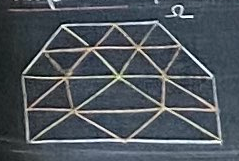
\includegraphics[width=1\textwidth]{images/diskretizace.png}
        \caption{Diskretizace $\Omega$ \hfill\break Bíla je původní oblast,\hfill\break žlutě základní rozdělení,\hfill\break červeně zjemnění \hfill}
    \end{subfigure}
    \hfill
    \begin{subfigure}[t]{0.3\textwidth}
        \centering
        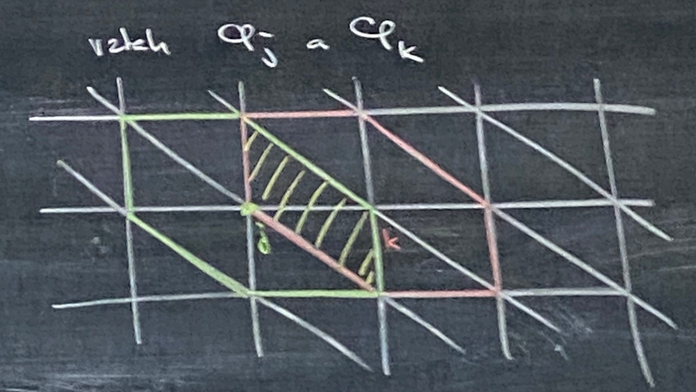
\includegraphics[width=1\textwidth]{images/vztahphi.png}
        \caption{Vztah $\phi_j$ a $\phi_k$}
    \end{subfigure}
    \hfill
    \begin{subfigure}[t]{0.3\textwidth}
        \centering
        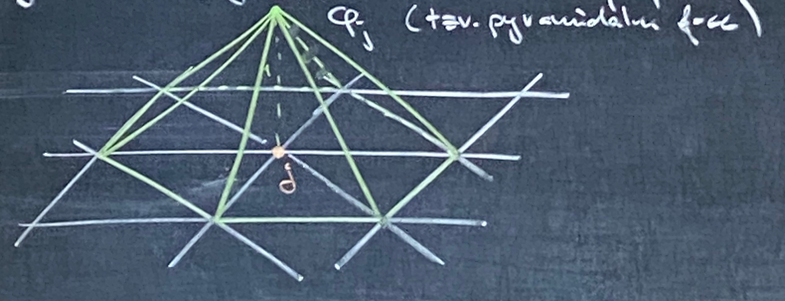
\includegraphics[width=1\textwidth]{images/grafphi.png}
        \caption{Graf funkce $\phi_j$}
    \end{subfigure}
\end{figure}

\end{document}